\documentclass[a4paper,12p]{scrreprt}
\usepackage[left= 2.5cm,right = 2cm, bottom = 4 cm]{geometry}

% Standard Packages
\usepackage[utf8]{inputenc}
\usepackage[ngerman]{babel}
\usepackage[T1]{fontenc}
\usepackage{graphicx, subfig}
\usepackage{subcaption}
\usepackage{fancyhdr}
\usepackage[backend=biber]{biblatex}
\usepackage{listings}
\usepackage{xcolor}
\usepackage{float}
\addbibresource{references.bib}
\usepackage{enumitem}
\usepackage{mathptmx}
%\usepackage{lmodern}
%\usepackage{color}

%Für Usepackage Lisiting -> ermöglicht Code einzufügen:
\lstset{ 
  language=[Sharp]C,
  basicstyle=\small\ttfamily, % Kleine Schriftgröße für den Code
  keywordstyle=\color{blue},
  commentstyle=\color{green!40!black}, % Dunklere Grüntöne für Kommentare
  stringstyle=\color{orange},
  numbers=left,
  numberstyle=\tiny,
  numbersep=5pt,
  breaklines=true,
  showspaces=false,
  showstringspaces=false,
  frame=none,
  rulecolor=\color{black},
  captionpos=b
}



% zusätzliche Schriftzeichen der American Mathematical Society
\usepackage{amsfonts}
\usepackage{amsmath}

% Für Abkürzungsverzeichniss
\usepackage[]{acronym}

% Begin des Dokumenntes
\begin{document}

\renewcommand{\thechapter}{\roman{chapter}}

\begin{figure}[h]
    \centering
    
\includegraphics[width = 0.55\textwidth]{img/Image_OTH.jpg}
    \label{fig: OTH Image}
\end{figure}


\begin{center}
    {\Huge {Vertiefung Microcomputertechnik} }
\end{center}

\vspace{2cm}

\noindent\makebox[\linewidth]{\rule{\linewidth}{0.4pt}}
\begin{center}
    {\Huge\textbf{CAN-TO-GO-SYSTEM} }
\end{center}
\noindent\makebox[\linewidth]{\rule{\linewidth}{0.4pt}}

\vspace{2cm}

\begin{center}
    {\Large {Von Michael Graml und Leonard Kreil} }
\end{center}

\vspace{1cm}

\begin{center}
    {\Large {Betruer/Prüfer: Prof. Dr. Stefan Krämer\\

             }}
\end{center}

\vspace{5cm}

\begin{center}
    {\Large Abgabe: 12.02.2024}
\end{center}

\newpage
\pagenumbering{Roman}
%Ab jetzt mit Kopf und Fußzeile
% ============= Kopf- und Fußzeile =============
\pagestyle{fancy}

%
\lhead{}
\chead{}
\rhead{\slshape \leftmark}
%%
\lfoot{Bachelorarbeit}
\cfoot{Leonard Kreil}
\rfoot{\thepage}
%%
\renewcommand{\headrulewidth}{0.4pt}
\renewcommand{\footrulewidth}{0.4pt}

%\include{02_Sperrvermerk_Erklärung}
%\include{03_Zusammenfassung}
\addsec{Zusammenfassung / Abstract}
\label{sec:zusammenfassung}
Das ist meine Zusammenfassung

\minisec{Abstract}
\label{abstract}

lalalal

%Inhaltsverzeichnis
\include{10_Abkürzungsverzeichniss}
\tableofcontents
\thispagestyle{fancy}
\pagenumbering{arabic} % Wechsel zu arabischen Seitenzahlen
\renewcommand{\thechapter}{\arabic{chapter}} % Ändert die Kapitelnummerierung auf römische Ziffern



%\include{07_CPCOM}
\chapter{Einleitung}
\label{sec:Einleitung}
\noindent Die Arbeit wurde gemeinschaftlich von Michael Graml und Leonard Kreil durchgeführt. Sollten Unterschiede in der Bearbeitung einzelner Abschnitte vorliegen, sind diese in den jeweiligen Kapiteln gekennzeichnet.\\

\begin {centering}
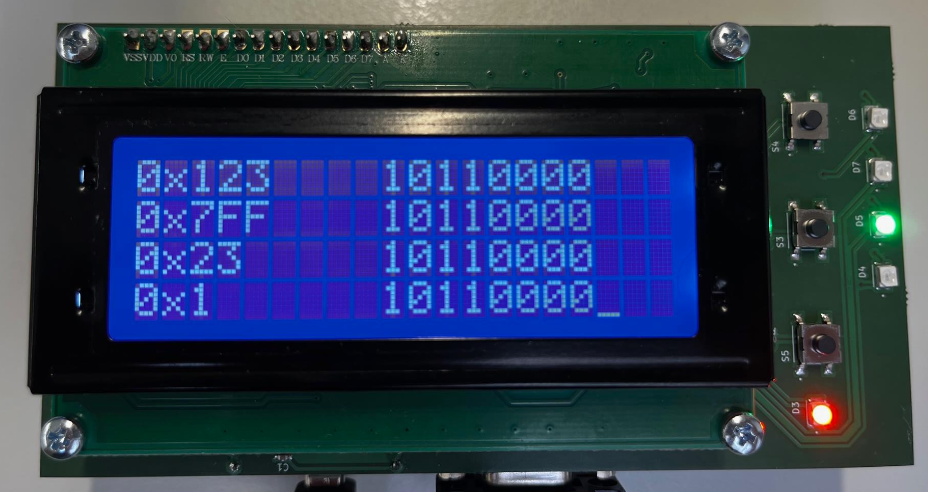
\includegraphics[width=0.75\textwidth]{img/Can_to_go_system.png}
\captionof{figure}{CAN-TO-GO System}
\label{fig: CAN-to-go System}
\end {centering}  


\section{CAN}
Controller Area Network (CAN) ist ein standardisiertes, robustes Fahrzeugbussystem, das für die Kommunikation zwischen verschiedenen Steuergeräten (ECUs) in Fahrzeugen und anderen industriellen Anwendungen konzipiert wurde. Es ermöglicht den zuverlässigen Datenaustausch mit hoher Fehlertoleranz und geringer Latenz, was besonders in Echtzeitanwendungen wichtig ist. CAN-Busse verwenden ein Nachrichtenbasiertes Protokoll, bei dem jede Nachricht eine eindeutige ID hat, die ihre Priorität bestimmt. Dieses System ist besonders nützlich bei der Diagnose von Netzwerkproblemen, da die Priorisierung von Nachrichten und Fehlererkennungsmechanismen die Fehlersuche erleichtern. Die physikalischen Aspekte des CAN-Busses, wie Abschlusswiderstände und die Verkabelung (CANL/CANH), sind ebenfalls entscheidend für die Netzwerkintegrität. Die Anpassungsfähigkeit hinsichtlich der Baudrate und die Unterstützung verschiedener Netzwerkstrukturen machen CAN vielseitig einsetzbar.\\

\section{Can-Datentelegram}
\begin{figure}[h]
    \centering
    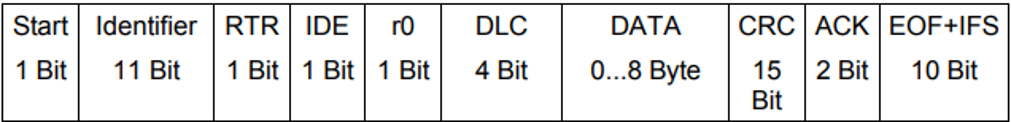
\includegraphics[width = 0.55\textwidth]{img/standard_datenframe.png}
    \caption{Standard Datentelegram \cite{3}}
    \label{fig: Standard Datentelegram}
\end{figure}
\begin{figure}[h]
    \centering
    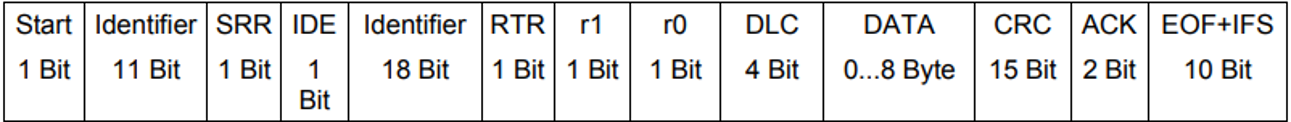
\includegraphics[width = 0.55\textwidth]{img/extended_datenframe.png}
    \caption{Extended Datentelegram \cite{3}}
    \label{fig: Extended Datentelegram}
\end{figure}

\noindent Ein CAN-Datentelegramm beginnt mit einem Startbit zur Synchronisation der kommunizierenden Geräte. Der Identifier gibt die Nachrichtenpriorität an und dient der Busarbitrierung, wobei das RTR-Bit zwischen einem Daten- und einem Datenanforderungstelegramm unterscheidet. IDE ist die Identifier Extension, die anzeigt, ob ein Standard- (11-Bit-Identifier siehe Abbildung \ref{fig: Standard Datentelegram}) oder ein Extended-Frame (29-Bit-Identifier siehe Abbildung \ref{fig: Extended Datentelegram}) verwendet wird. DATA enthält die eigentlichen Nutzdaten. CRC ist eine Prüfsumme zur Fehlererkennung. ACK signalisiert den korrekten Empfang der Nachricht. EOF und IFS kennzeichnen das Ende des Datentelegramms und den erforderlichen Abstand bis zum nächsten Frame. Im Extended Frame ersetzt das SRR-Bit das RTR-Bit des Standard Frames, und die DLC-Information gibt die Länge der Daten an.\\

\section{Anfordderungsanalyse}
\noindent Das "Can to Go"-System wird entwickelt, um Anwendern bei Problemen beim Aufbau eines CAN-Busses zu assistieren und zu diagnostizieren, wo genau die Schwierigkeiten liegen. Es dient als funktionssicherer CAN-Teilnehmer, der in der Lage ist, CAN-Nachrichten zuverlässig zu lesen und zu interpretieren. Kernmerkmale umfassen ein Anschlusskästchen mit SUB-D-Stecker und Status-LEDs, die den Betriebszustand des CAN-Busses anzeigen. Ein optionaler Abschlusswiderstand, der nach Bedarf zugeschaltet werden kann, sowie die Anpassungsfähigkeit der Baudrate gehören ebenfalls zu den wesentlichen Anforderungen. Darüber hinaus wird das System die CAN-Nachrichten und die zugehörigen Sender-IDs sichtbar machen.\\


\section{Endprodukt}

\subsection{Überblick}
\noindent Das Endprodukt des "Can to Go"-Systems bildet eine fortschrittliche Lösung für die Überwachung und Diagnose von CAN-Bussystemen. Es integriert die erforderlichen Funktionen aus der Anforderungsanalyse mit zusätzlichen Merkmalen, die seine Benutzerfreundlichkeit und Vielseitigkeit erhöhen.\\

\subsection{Hauptmerkmale}
\begin{itemize}
    \item \textbf{Anschluss und Konnektivität:} Ausgestattet mit einem Anschlusskästchen und SUB-D-Stecker, verfügt das System über Status-LEDs, die den Betriebszustand des CAN-Busses anzeigen. Diese visuellen Indikatoren erleichtern das schnelle Erkennen von Verbindungsproblemen.
    
    \item \textbf{Funktionalität und Anpassungsfähigkeit:} Ein optionaler Abschlusswiderstand kann nach Bedarf hinzugeschaltet werden. Die Anpassbarkeit der Baudrate gewährleistet eine breite Kompatibilität mit verschiedenen CAN-Bus-Konfigurationen.
    
    \item \textbf{Display und Anzeige:} Das Gerät umfasst ein kleines Display, das CAN-Nachrichten anzeigt. Dieses Display bietet eine direkte, wenn auch begrenzte, Einsicht in die CAN-Kommunikation.
    
    \item \textbf{Energieversorgung:} Es enthält keinen eigenen Akku, kann aber durch eine externe Powerbank mit Energie versorgt werden, was eine flexible Nutzung ermöglicht.
\end{itemize}   

\subsection{Zusätzliche Funktionen}
\begin{itemize}
 \item \textbf{App- und Web-Integration:} Ergänzend zum kleinen Display des Geräts ermöglichen eine App und eine Website die detaillierte Ansicht von CAN-Nachrichten, inklusive Zeitstempeln. Diese digitalen Plattformen erlauben eine umfassende Analyse da sie eine größere Benutzeroberfläche als das Display bieten.
\end{itemize}   





% Verzeichnis der Quellen
\printbibliography
% Verzeichnis der Bilder
\listoffigures
% Verzeichnis der Listings
\lstlistoflistings

\end{document}